\label{subsec:precision_timing_inst_ptarm}

%mention that a full scaled worst case execution time analysis is beyond the scope of this thesis.
%but do a brief summary on how it's done, cite wilhelm's group's research summary
Worst-case execution time (WCET) analysis is a combined analysis of the control paths that the software might exhibit, and the time it takes to execute those paths on the underlying architecture. 
A plethora of research has been done on the software analysis of control paths. 
Wilhelm et al.~\cite{wilhelm-survey-paper} presented a survey of tools and techniques available for worst-case path enumeration and loop analysis etc.
However, the precision of the WCET analysis of those techniques ultimately depend on the underlying architecture implementation~\cite{Heckmann2003processor}.
Architectures that exhibit wildly unpredictable execution times will result in overly conservative WCET analysis, even if the software structure is simple. 
Designed as a predictable architecture, the instructions of PTARM all exhibit deterministic timing behaviors, allowing a more precise WCET as software analysis progresses. 
In section~\ref{sec:ptarm_instructions} we discussed the implementation of each instruction and explained the execution time of each instruction type.
Table~\ref{table:ptarm_instruction_timing} summarizes the execution time each instruction takes in terms of \emph{thread cycles}. 

A \emph{Thread cycle} is the unit used to represent execution time on each thread.  
Timing analysis can be done separately for each hardware thread running on PTARM because the threads are temporally isolated; the execution time of each thread cannot be affected by other threads.
The thread-interleaved pipeline switches thread contexts every processor cycle in a predictable round robin fashion. 
Thus, each thread is fetched and executed in the pipeline every $N$ processor cycles, $N$ being the number of threads in the pipeline.
One \emph{Thread cycle} represents each time the thread enters in the pipeline, which is the thread's perceived notion of cycles.
The execution frequency of each thread ($F_{thread}$) is $F_{thread} = F_{processor}/N$, so each \emph{thread cycle} is $1/F_{thread}$ long. 
For example, our PTARM core is clocked at 100$MHz$ ($F_{processor} = 100 * 10^6$) and has 4 threads ($N=4$) , so each thread cycle is $1/((100 * 10^6)/4) = 40 * 10^{-9}$ secs, or 40 nanoseconds long.
The length of the \emph{thread cycle} will not change because of the predictable thread-switching policy, making it a reliable unit of measurement for execution time.   

\begin{table}
\noindent\makebox[\textwidth]{%
\begin{smalltabular}{ | p{4cm} | c || p{9cm} | }
  \hline                        
  \textbf{Instruction Type} & \textbf{Thread Cycles} & \textbf{Notes}    \\ \hline
  Data Processing  & 1 & \multirow{2}{9cm}{ ${\ast}$: an additional cycle is added if pre or post-index offset is used in the address mode.}  \\ \cline{1-2} 
  Branch  & 1 &  \\ \cline{1-2}
  Load/Store (SPM)  & 1$^{\ast}$ &  \multirow{4}{9cm}{ ${\phi}$: the dram latency is 3 or 4 thread cycles depending on the alignment of the pipeline and the dram controller backend, as described in section~\ref{sec:ptarm_dram_integration}. For conservative estimates, 4 thread cycles is used. } \\ \cline{1-2} 
  Load/Store (BootROM)  & 1$^{\ast}$ & \\ \cline{1-2}  
  Load/Store (DRAM) & 4$^{\phi \dagger \ast}$ & \\ \cline{1-2}
  Load/Store Multiple & $N_{reg} \times L_{mem}$ $^{\Delta \ast}$ &  \\  \cline{1-2}
  Software Interrupt (SWI) & 1 & \multirow{4}{9cm}{ ${\dagger}$: a single store buffer is implemented, as described in section~\ref{sec:ptarm_dram_store_buffer}, so non-consecutive stores take only 1 thread cycle, while consecutive stores require the full dram latency of 3 or 4.}\\    \cline{1-2}
  get\_time  & 2 &  \\ \cline{1-2}
  delay\_until  & 1 $^{\sigma}$ & \\    \cline{1-2}
  exception\_on\_expire  & 1  &    \\   \cline{1-2}
  deactivate\_exception & 1 &  \multirow{2}{9cm}{ ${\Delta}$: $N_{reg}$ is number of registers specified in the instruction. $L_{mem}$ is the latency of the memory region operated on.} \\  \cline{1-2}
  \multicolumn{2}{|c|}{} &  \\ \cline{1-2}
  \multicolumn{2}{|c|}{} &   \multirow{2}{9cm}{${\sigma}$: denotes the minimum execution time. Actual execution time depends on the system clock and the specified deadline.} \\ \cline{1-2}
  \multicolumn{2}{|c|}{} &\\ \hline
\end{smalltabular}}
\caption{Timing properties of PTARM instructions}
\label{table:ptarm_instruction_timing}
\end{table}

\subsection{Memory instructions}
Data-processing instructions typically have straightforward execution times on most architectures.
In our case, branch instructions also have very a predictable and straightforward execution, as the branch penalty is completely hidden within the thread interleaving.
The memory instructions in our architecture however can have several different latencies depending on addressing mode or region of access, as listed in table~\ref{table:ptarm_instruction_timing}.
For memory instructions that use pre or post-indexed addressing mode to update the base register, an additional cycle latency is needed to write back to the base register, as described in the instruction implementation in section~\ref{sec:ptarm_instruction_ldstr}.
But the addressing mode of load/store instructions can be determined statically, as it is part of the instruction encoding, so it does not affect the complexity or precision of execution time analysis. 

For load instructions, the exposed memory hierarchy allows us to clearly label and identify access latencies to different memory regions.
In execution time analysis, value analysis attempts to determine what memory addresses are accessed.     
In systems that use caches and hide the memory hierarchy, additional modeling of the cache state is still needed after the value analysis determines the potential memory addresses that are accessed.
However, with an exposed memory hierarchy with scratchpads, the precision of execution time analysis depends only on the value analysis. 
As soon as the memory address is determined, we can give a associate a precise memory access latency.
The worst-case DRAM latency of 4 thread cycles is derived from~\cite{ReinekeLiuPatelKimLee11_PRETDRAMControllerBankPrivatizationForPredictability}. 
This allows not only for a simpler timing analysis, but also a more accurate analysis.

For store instructions, the single store buffer as described in section~\ref{sec:ptarm_dram_store_buffer} can possibly hide the latency of store instructions if no other memory access instruction comes after it. 
Otherwise the store instruction will take the full memory access latency, depending on the memory access region of the store.
Timing analysis tools can mostly account for the store buffer by statically checking a few instructions ahead of the store instruction to see if there are memory accessing instructions.
The window of instructions that need to be checked is very narrow, so it should not really complicate the analysis.
If this is not possible, then conservatively, the full memory access latency should be used for each store, depending on the access region.

The execution time of load/store multiple instructions depend on the number of registers operated on, and the memory region it accesses. 
Because the register list is statically encoded in the instruction, the number of registers operated on can easily be statically determined.
Store multiple instructions do not benefit from the store buffer, so all accesses take the full memory access latency.
For each register that is operated on, the latency will depend on which memory region it accesses. 
The total execution time of the instruction will be the sum of the latencies for all register operations. 
If pre or post-indexed addressing mode is used, an extra cycle is added to update the base register, just as regular load/store instructions. 

\subsection{Timing instructions}
Even though the execution time of most timing instructions can be statically determined, they impact the execution time of the program in a very dynamic way.
For example, the execution of \exceptiononexpire\ and \deactivateexception\ only take one cycle, but when the \timerexpired\ exception is thrown, the execution time of the whole program is affected. 
To understand the timing effects of the timing instructions, we must understand the implementation effects on the precision of the timing instructions.
It is impossible for any hardware implementation to provide absolute precision of time, as we are limited by the precision of the digital synchronous circuits that discretize the notion of time. 
Although the timing extensions allow the manipulation of nanoseconds in software, with the thread-interleaved pipeline, the basic unit of time for each thread is one thread cycle, or 40 nanoseconds, in PTARM.
As a result, 40 nanoseconds is the shortest interval of time that is observable by each thread.
This can also be explained from the implementation of the pipeline.
Each thread only latches the timer value in the fetch stage, and the timestamp is propagated along the pipeline and associated with the instruction. 
Since there are four threads cycling in a round robin fashion, each thread latches the timer value only once every 4 processor cycles. 
With 100MHz clocking the pipeline in our implementation, 4 processor cycles is  equivalent to 40 nanoseconds. 

When setting deadlines, the execution time of the timing instructions must be taken into account. 
As explained in the implementation, each timing instruction latches the current platform time in the fetch stage.
That timestamp is used throughout instruction execution and associated as the current time.  
For example, the time value in the timestamp obtained from \gettime\ will contain the time before the execution of \gettime.
Since \gettime\ takes 2 thread cycles every execution, 80 nanoseconds will have elapsed when the timestamp is obtained from \gettime.
In the same way, \delayuntil\ latches the current platform time at the fetch stage each thread cycle, and compares with the input timestamp. 
\Delayuntil\ will delay program execution until the latched platform time is \emph{greater than or equal to} the input timestamp value.
So when \delayuntil\ completes its execution, the current platform time will be \emph{at least} 40 nanoseconds greater than the input timestamp specified, to account for the execution of \delayuntil. 

\begin{figure}[h]
  \begin{center}
    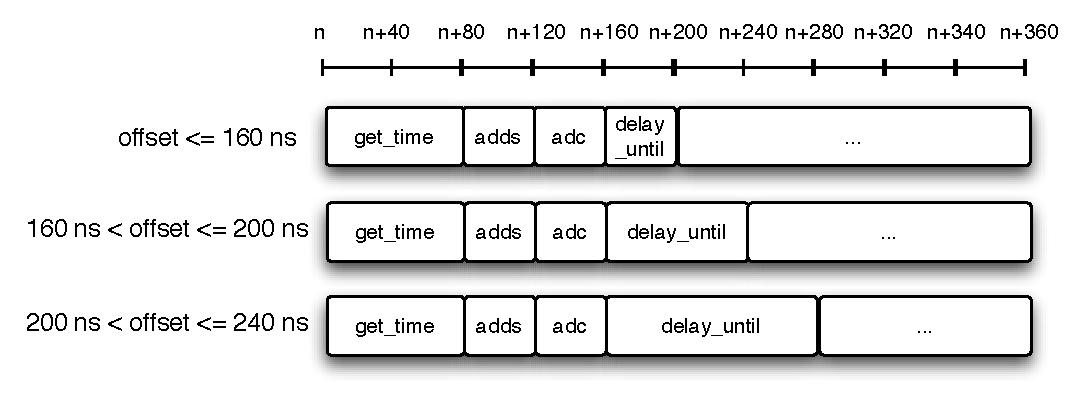
\includegraphics[scale=.7]{figs/delay_until_details}
  \end{center}
  \vspace{-3mm}
  \caption{Timing details of get\_time and delay\_until}
  \label{fig:delay_until_details}
\end{figure}

\todo{make figure for exception on expire!}

Figure~\ref{fig:delay_until_details} illustrates this effect by showing a timeline of execution for one thread on PTARM. 
The code segment starts executing at time $n$. 
The code only consists of \gettime, \delayuntil, and 2 add instructions used to add an offset to the timestamp obtained by \gettime.
For all 3 cases, the timestamp obtained by \gettime\ would contain the value $n$, even though the instruction after \gettime\ executes at $n+80$.
Taking into account the 2 thread cycles used to add the offset to the timestamp, if the offset is $\leq 160$, then the \delayuntil\ will simply serve as a NOP. 
This is because when \delayuntil\ is executed, it will latch $n+160$ for the platform time, and it will only delay program execution if the input timestamp is $> n+160$.
This is shown in the top case of the figure.
Notice that the instruction after \delayuntil\ executes at time $n+200$, which accounts for the 1 thread cycle it takes to execute \delayuntil.
Assuming \delayuntil\ does delay the program, in the worst-case, the instruction after \delayuntil\ executes $79 ns$ after the input timestamp. 
This can be observed if the offset is set to 161, which will result in the middle timeline shown in figure~\ref{fig:delay_until_details}.  
\Delayuntil\ will first latch the time $n+160$ to compare with the input timestamp of $n+161$. 
Because current platform time is less than input timestamp, \delayuntil\ will delay the execution of the program until the next cycle, when $n+200$ is latched to be checked against the input timestamp. 
At that point, \delayuntil\ will complete its execution, and the next instruction will execute at $n+240$.
This jitter results from the minimum observable time interval of $40 ns$ for each thread, causing \delayuntil\ to have an observable jitter of up to $40 ns$. 
\subsection{Timed Loop revisited}
We give a concrete example of analysis of timing instructions on PTARM by deriving the \emph{offset} from the self compensating timed loop shown in section~\ref{sec:timed_loops}.
This timed loop detects whether the previous loop iteration missed its deadline. 
If it did, then the current iteration will execute a shorter version of the task in attempt to make up for the lost time, as shown in figure~\ref{fig:self_compensating_loop_timing}.  
\begin{figure}[h]
  \vspace{-3mm}
  \begin{center}
    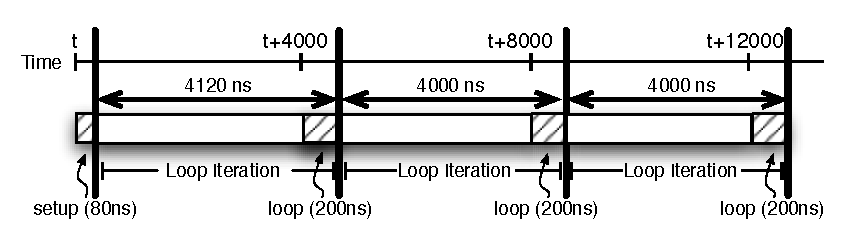
\includegraphics[scale=.7]{figs/self_compensating_loop_timing}
  \end{center}
  \vspace{-3mm}
  \caption{Execution of the self compensating timed loop}
  \label{fig:self_compensating_loop_timing}
\end{figure}
\vspace{-8mm}
\begin{lstlisting}[float=h, label=lst:timed_loop_compensate_revisit,caption=Timed loops with compensation revisited]
  cdp p13, 8, c2, c0, c0, 0  ; get_time, deadline timestamp stored in [c2, c3]
loop:
  cdp p13, 8, c4, c0, c0, 0  ; get_time, current timestamp stored in [c4, c5]
  subs r5, r5, #80           ; compensate for loop overhead and delay_until 
  sbc  r4, r4, #0            ; 

  subs r3, r3, r5            ; Check if previous iteration deadline is missed
  sbc  r2, r2, r4            ; 

  blmi task_short            ; execute shorter task if previous deadline mess 
  blpl task_normal           ; or else execute normal task 
  
  adds r3, r3, #4000         ; assuming the deadline is 4 us (4000 ns)
  adc r2, r2, #0             ; calculate the deadline timestamp for this iter.
  cdp p13, 4, c2, c2, c3, 0  ; delay_until
   
  b loop
\end{lstlisting}

\subsubsection{Obtaining the offset}
Listing~\ref{lst:timed_loop_compensate_revisit} shows the source code that is used to construct this timed loop. 
During the miss detection (lines 3 to 8), an additional \textit{offset} is used to compensate for the execution of \delayuntil\ and loop overhead.
Time elapses between the \delayuntil\ of the previous loop iteration (line 15), where the previous deadline timestamp is checked, and the \gettime\ used for miss detection (line 3) in the current iteration.
Without the offset compensation, the loop overhead will cause the miss detection to always detect a missed deadline.
This can be observed from table~\ref{table:timed-loop-compensate-timing}, where we show a sample execution trace of four iterations in this timed loop.  
Figure~\ref{fig:self_compensating_loop_timing} shows the timing behavior of these four iterations, where a missed deadline in the second iteration will cause the third iteration to compensate by executing the shorter version of the task.

\begin{table}
\vspace{-5mm}
\begin{center}
\noindent\makebox[\textwidth]{%
\begin{smalltabular}{ | l | l | l r | }
  \hline
  \textbf{Time} & \textbf{TC} & \textbf{Instruction} & \textbf{Comment}\\ \hline \hline 
  t ns & n &  \textit{cdp p13, 8, c2, c0, c0, 0} & get\_time (deadline: t) \\  \hline
  \multicolumn{4}{|c|}{ -- -- Loop 1st iteration / No deadline miss -- -- } \\ \hline    
  t+80 ns & n+2 &  \textit{cdp p13, 8, c4, c0, c0, 0 } & get\_time, (current: t+80) \\
  t+160 ns & n+4 &  \textit{subs r5, r5, \#80} & (current -= 80)\\
  t+200 ns & n+5 &  \textit{sbc  r2, r2, r4} & (current: t)\\  
  t+240 ns & n+6 &  \textit{subs r3, r3, r5} & compare deadline (t) and current (t) \\
  t+280 ns & n+7 &  \textit{sbc  r2, r2, r4} & result is 0, clear cc[``n''] \\
  t+320 ns & n+8 &  \textit{blmi task\_short} & nop since cc[``n''] == 0\\
  t+360 ns & n+9 &   \textit{blpl task\_normal} & branch since cc[``n"] == 0\\  
    - ns & - &  \ldots & executing task\_normal \\  
  t+3800 ns & n+95 & \textit{adds r3, r3, \#4000} &  (deadline += 4000) \\
  t+3840 ns & n+96 & \textit{adc r2, r2, \#0} &  (deadline: t+4000) \\ 
  t+3880 ns & n+97 &  \textit{cdp p13, 4, c2, c2, c3, 0} & delay\_until, input timestamp is t+4000\\
  - ns & - & \ldots & delay\_until for 3 thread cycles\\  
  t+4040 ns & n+101 &  \textit{b loop} & jump back to loop \\ \hline
  \multicolumn{4}{|c|}{ -- -- Loop 2nd iteration / Deadline miss -- -- } \\ \hline    
  t+4080 ns & n+102 &  \textit{cdp p13, 8, c4, c0, c0, 0 } & get\_time, (current: t+4080)\\
  t+4160 ns & n+104 &  \textit{subs r5, r5, \#80} & (current -= 80)\\
  t+4200 ns & n+105 &  \textit{sbc  r2, r2, r4} & (current: t+4000)\\  
  t+4240 ns & n+106 &  \textit{subs r3, r3, r5} & compare deadline (t+4000) and current (t+4000)\\
  t+4280 ns & n+107 &  \textit{sbc  r2, r2, r4} & result is 0, clear cc[``n''] \\
  t+4320 ns & n+108 &  \textit{blmi task\_short} & nop since cc[``n''] == 0\\
  t+4360 ns & n+109 &   \textit{blpl task\_normal} & branch since cc[``n"] == 0\\  
  - ns & - &  \ldots & code for task\_normal \\  
  t+7960 ns & n+199 & \textit{adds r3, r3, \#4000} & (deadline += 4000) \\
  t+8000 ns & n+200 & \textit{adc r2, r2, \#0} & (deadline: t+8000) \\ 
  t+8040 ns & n+201 &  \textit{cdp p13, 4, c2, c2, c3, 0} & delay\_until, *no delay*\\
  t+8080 ns & n+202 &  \textit{b loop} & jump back to loop \\ \hline
  \multicolumn{4}{|c|}{ -- -- Loop 3rd iteration / Compensate with shorter task -- -- } \\ \hline    
  t+8120 ns & n+203 &  \textit{cdp p13, 8, c4, c0, c0, 0 } & get\_time, (current: t+8120)\\
  t+8200 ns & n+205 &  \textit{subs r3, r3, r5} & (current -= 80)\\
  t+8240 ns & n+206 &  \textit{sbc  r2, r2, r4} & (current: t+8040) \\
  t+8280 ns & n+207 &  \textit{subs r3, r3, r5} & compare deadline (t+8000) and current (t+8040)\\
  t+8320 ns & n+208 &  \textit{sbc  r2, r2, r4} & result is -40, set cc[``n''] \\
  t+8360 ns & n+209 &  \textit{blmi task\_short} & branch since cc[``n"] == 1 \\
  - ns & - &  \ldots & code for task\_short \\  
  t+10280 ns & n+257 &   \textit{blpl task\_normal} & nop since cc[``n''] == 1\\    
  t+10320 ns & n+258 & \textit{adds r3, r3, \#4000} & (deadline += 4000) \\
  t+10360 ns & n+259 & \textit{adc r2, r2, \#0} & (deadline: t+12000) \\ 
  t+10400 ns & n+260 &  \textit{cdp p13, 4, c2, c2, c3, 0} & delay\_until\\
  - ns & - &  \ldots & delay until time is t+12000 \\  
  t+12040 ns & n+301 &  \textit{b loop} & jump back to loop \\ \hline
   \multicolumn{4}{|c|}{ -- -- Loop 4th iteration / Execute normal task -- -- } \\ \hline    
  t+12080 ns & n+302 &  \textit{cdp p13, 8, c4, c0, c0, 0 } & get\_time, (current: t+12080)\\
  t+12160 ns & n+304 &  \textit{subs r3, r3, r5} & (current -= 80)\\
  t+12200 ns & n+305 &  \textit{sbc  r2, r2, r4} & (current: t+12000) \\
  t+12240 ns & n+306 &  \textit{subs r3, r3, r5} & compare deadline (t+12000) and current (t+12000)\\
  t+12280 ns & n+307 &  \textit{sbc  r2, r2, r4} & result is 0, clear cc[``n''] \\
  \hline 
\end{smalltabular}}
\end{center}
\vspace{-3mm}
\caption{Instruction execution trace of the self compensating timed loop\\ (TC = thread cycles)}
\label{table:timed-loop-compensate-timing}
\end{table}

In table~\ref{table:timed-loop-compensate-timing}, execution starts at time $t$.
As mentioned before, each thread cycle is $40ns$, which is reflect in the left most column that shows the progression of time.
We also show the thread cycle (TC) count, which starts at $n$ when execution begins.
The execution time of each instruction is according to table~\ref{table:ptarm_instruction_timing}.
In this code segment, we keep track of two timestamps each iteration. 
The \emph{deadline\_timestamp} keeps track of the loop deadlines, and is stored in registers r2 and r3.  
The \emph{current\_timestamp} is updated with \gettime\ in the beginning of each loop iteration to detect if the previous iteration missed its deadline.
It is stored in registers r4 and r5. 
The loop period is set to be $4 \mu s$, which is $4000 ns$ (100 thread cycles).
We add the loop period to the \emph{deadline\_timestamp} each loop iteration (lines 13 and 14 in the listing).  

\newcommand{\currentt}{\emph{current\_timestamp}}
\newcommand{\deadlinet}{\emph{deadline\_timestamp}}


The need for the \emph{offset} can be observed at the beginning of the second loop iteration.
At time $t+4080ns$, \gettime\ is called to initiate the miss detection sequence.
The previous \deadlinet\ is $t+4000$, which was met in the first iteration.  
However, \gettime\ updates the \currentt\ to $t+4080$, because the execution of \delayuntil\ and \emph{b loop} took 2 thread cycles combined. 
Thus, our miss detection accounts for this by subtracting the 2 thread cycles ($80ns$) overhead from \currentt\ before comparing it with \deadlinet.
In general, the overhead that needs to be account for is the time elapsed between the deadline checking \delayuntil\ instruction and the miss detection \gettime\ instruction.
Intuitively this is because we want to check whether the previous \delayuntil\ executed before the previous \deadlinet, so the \emph{offset} is used to calculate the time of execution of the previous \delayuntil.  

\subsubsection{Overhead of the self compensating timed loop}
In this self compensating timed loop, the loop period is set to $4000ns$, and regulated with the \delayuntil\ instruction.
However, the loop period includes the execution of the actual task along with the loop and timing control overhead.
The loop overhead in this example is only the branch instruction on line 17 in listing~\ref{lst:timed_loop_compensate_revisit}, which is 1 thread cycles (40 ns).
The overhead for timing control and self compensation consists of all the timing instructions, the arithmetic on the timestamps, and the 2 conditional branch instructions that determines which task to execute.
From table~\ref{table:timed-loop-compensate-timing} we can count a total overhead of 11 thread cycles including 1 \gettime\ (2 thread cycles), 1 \delayuntil\ (1 thread cycle), 6 arithmetic operations on the timestamps (6 thread cycles), and 2 conditional branch instructions (2 thread cycles).
Overall the timed loop contains an overhead of 12 thread cycles ($480ns$) , which means the executed tasks (both normal and short) have a timing requirement of 88 thread cycles ($3520ns$) in order for each loop iteration to meet its deadline.  
In the second loop iteration for our example, \emph{task\_normal} executed for 89 thread cycles, exactly one thread cycle over its timing requirement. 
As a result, the \delayuntil\ of the second loop iteration did not delay program execution, and the third iteration miss detection detects a missed deadline, and switches to execute \emph{task\_short}. 

\subsubsection{First loop iteration jitter}
The \emph{offset} previously derived is an overhead that is executed in every iteration of the loop.
In our code, the overhead only included the execution time of the \delayuntil\ and a branch, as we always unconditionally branch to the beginning of the loop. 
However, if the overhead was larger, for example, in a conditional loop structure, then it could introduce jitter for the first iteration.
An example is shown in figure~\ref{fig:setup_look_timing}, where we used an overhead of 200ns, instead of 80ns.
\begin{figure}[h]
  \vspace{-3mm}
  \begin{center}
    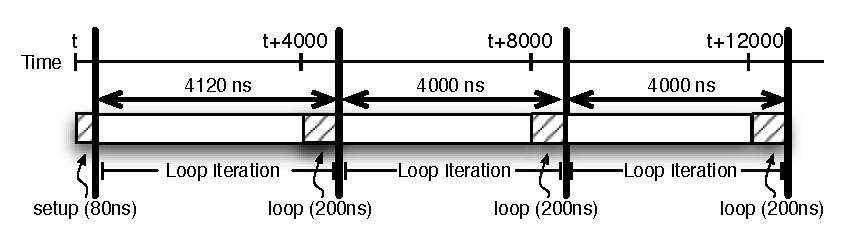
\includegraphics[scale=.9]{figs/setup_loop_timing}
  \end{center}
  \vspace{-3mm}
  \caption{Jitter caused by initial timed loop setup}
  \label{fig:setup_look_timing}
\end{figure}
We assume that the setup code remains the same with only one \gettime, and the \emph{offset} is adjusted to 200ns for the miss detection.
We also assume that the loop periond remains the same, 4000ns, and all loop iterations meet the loop period timing requirements. 
In this example, we see that the first iteration executes for 120ns longer than subsequent iterations.
The jitter for the first iteration is introduced by the execution time difference between the \emph{offset} and the setup code.  
Between the \delayuntil\ instructions, exactly 4000 ns elapses, because 4000 ns is added to the \deadlinet\ each loop iteration.   
The execution of the overhead is included within the 4000 ns, except for the first iteration. 
Instead, between the initial \deadlinet\ and the first \delayuntil, the only overhead that is observed is the execution of a \gettime\ instruction, which is 80 ns. 
Thus, the first iteration of the loop executes for an addition 120ns, which is the difference between the \emph{offset} and the execution time of the loop setup code.
This effect was not observed by the previous example because the \emph{offset} and the loop setup both took 80 ns.
As a result, for the previous example, each loop iteration takes exactly 4000 ns if all loop deadlines were met.   

\begin{lstlisting}[float=h, label=lst:timed_loop_compensate_adj,caption=Jitter adjusted timed loop ]
  mov r6, #0                 ; i = 0;
  mov r7, #0                 ; j = 0;
  
  cdp p13, 8, c2, c0, c0, 0  ; get_time, deadline timestamp stored in [c2, c3]
  subs r3, r3, #40           ; adjustment for first loop period 
  sbc  r2, r2, #0            ; deadline -= 40
loop:
  cdp p13, 8, c4, c0, c0, 0  ; get_time, current timestamp stored in [c4, c5]
  subs r5, r5, #200          ; compensate for loop overhead and delay_until 
  sbc  r4, r4, #0            ; 

  subs r3, r3, r5            ; Check if previous iteration deadline is missed
  sbc  r2, r2, r4            ; 

  blmi task_short            ; execute shorter task if previous deadline mess 
  blpl task_normal           ; or else execute normal task 
  
  adds r3, r3, #4000         ; assuming the deadline is 4 us (4000 ns)
  adc r2, r2, #0             ; calculate the deadline timestamp for this iter.
  cdp p13, 4, c2, c2, c3, 0  ; delay_until
	
  add r6, r6, #1             ; i += 1    
  add r7, r7, r6 LSL #1      ; j += i*2  
  cmp r7, #1000              ; 
  blt loop                   ; branch back if ( j < 10000 )
\end{lstlisting} 

\begin{figure}[h]
  \vspace{-3mm}
  \begin{center}
    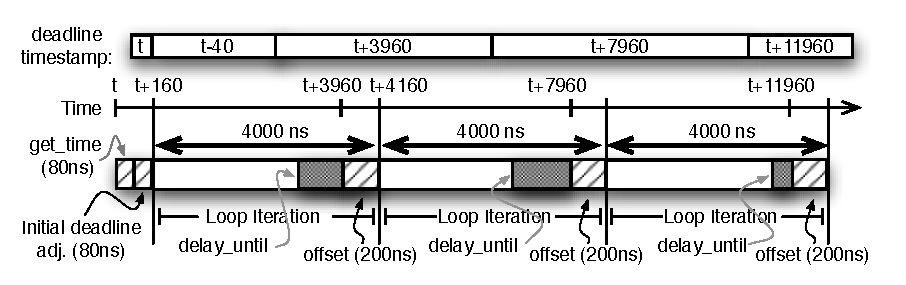
\includegraphics[scale=.9]{figs/setup_loop_timing_adj}
  \end{center}
  \vspace{-3mm}
  \caption{Adjusted timed loop setup}
  \label{fig:setup_look_timing_adj}
\end{figure}

This first iteration jitter can be accounted for by adjusting the initial \deadlinet\ in the loop setup code.
In listing~\ref{lst:timed_loop_compensate_adj} we show an example source code that adjusts for the additional overhead in the loop.
Lines 22 to 25 show the additional loop overhead that conditionally checks whether to branch back to the beginning of the loop.
The offset that we have to adjust for in this example is exactly 200ns, which includes the 4 instructions for the loop overhead and the \delayuntil. 
This offset is reflected on line 9.
Lines 4 to 6 show the loop setup code where we adjust for the execution time of the initial loop iteration, where 40 is subtracted from the initial \deadlinet\ obtained by the \gettime\ on line 4.
This value is obtained by the execution time difference of the overhead, which is $200ns$, and the setup code after \gettime, which is $160 ns$ (4 thread cycles).
We show the resulting timing behavior in figure~\ref{fig:setup_look_timing_adj}, where the first loop iteration is adjusted to 4000ns, the same as subsequent iterations.
By entering the loop with the \deadlinet\ value of $t-40$, we shift the \delayuntil\ deadlines for all loop iterations by 40 ns, allowing us to compensate for the first iteration jitter.   
Intuitively, we adjust the initial \deadlinet\ before entering the loop to create the illusion that the setup code and the loop overhead observed between each \delayuntil\ has the same execution time.
By doing so, the first loop iteration will observe the same loop period as all subsequent iterations. 

\subsection{Exceptions}
In section~\ref{subsec:exception_handling_in_ptarm} we described how exceptions are thrown in PTARM.
When an exception is triggered in one hardware thread, none of the other hardware threads are affected, as the pipeline is not flushed.
For the thread on which the exception occurred, only one thread cycle is lost, and the control flow jumps to the correct exception handler depending on the exception vector table.    
Here, we give a concrete example of the timing properties of exceptions on PTARM by showing how \exceptiononexpire\ and \deactivateexception\ trigger \timerexpired\ exceptions to handle missed deadlines immediately.
The code for the example is shown in listing~\ref{lst:exception-sample}.

\begin{lstlisting}[float=h, label=lst:exception-sample,caption=Sample code that triggers a \timerexpired\ exception ]
  mov  r3, #0x98              ; r3 = address of _timer_handler_loc 
  add  r4, pc, #32            ; r4 = addr of delay_handler
  str  r4, [r3]               ; register delay_handler
  
  cdp  p13, 8, c2, c0, c0, 0  ; get_time
  adds r3, #240
  adc  r2, #0
  cdp  p13, 2, c2, c2, c3, 0  ; exception_on_expire
  
  add  r5, r6, r6             ; arbitrary code block
  add  r7, r5, r6             ;
  
  cdp  p13, 5, c8, c2, c3, 0  ; deactivate_exception
  b end_program                       
  
delay_handler:
  mov pc, lr                  ; simply return
\end{lstlisting}

\newcommand{\delayhandler}{\emph{delay\_handler}}
\newcommand{\Delayhandler}{\emph{Delay\_handler}}
\newcommand{\timerhandlerloc}{\emph{\_timer\_handler\_loc}}

In this example, a \delayhandler\ is setup on lines 16 and 17 that simply returns when called.
\Delayhandler\ is registered as the exception handler for the \timerexpired\ exception, which happens on lines 1 to 3.
This is done by deriving the address of the \delayhandler\ on line 2, and storing it to the \timerhandlerloc.
The \timerhandlerloc\ is a reserved location that points to the address of the handler that is executed when the \timerexpired\ exception is thrown.
When a \timerexpired\ exception is thrown, the current address is saved and control flow jumps to the exception table entry for the \timerexpired\ exception.
This table entry redirects the execution to a \timerexpired\ exception setup code (shown in listing~\ref{lst:timer-expire-handler}) which calls the registered exception handler.
The setup code loads the address of \timerhandlerloc\ into a register, and jumps to the handler on line 7.
If the handler returns, lines 8 to 10 re-enable interrupts, and line 11 returns control to the original PC when the exception occurred.  
\begin{lstlisting}[float=h, label=lst:timer-expire-handler,caption=The \timerexpired\ exception setup code]
.text
.global _tmr_exp_setup;
_tmr_exp_setup:
    push  {r0, lr}
    ldr   r0, _timer_handler_loc 
    mov   lr, pc
    mov   pc, r0
    mrs   r0, cpsr
    bic   r0, r0, #0x80
    msr   cpsr, r0
    pop   {r0, pc}

_timer_handler_loc: .word  0x00000000;
\end{lstlisting}

The execution trace of this example is shown in table~\ref{table:exception-expire-timing}.
Because execution jumps back and forth between the main code, the \timerexpired\ setup code, and the \delayhandler, so we show the address of the instructions to help follow which code segment is being executed.   

\begin{table}[h]
\begin{center}
\noindent\makebox[\textwidth]{%
\begin{smalltabular}{ | c | c | l | l r | }
  \hline                        
  Time & TC & address & Inst & Comment\\ \hline
  t ns & n & 0x40000000 & \textit{mov r3, \#0x98} & get the timer handler address \\  
  t+40 ns & n+1 & 0x40000004 & \textit{add r4, pc, \#32} & get delay\_handler address \\
  t+80 ns & n+2 & 0x40000008 & \textit{str r4, [r3]} & register delay\_handler as timer expire handler\\
  t+120 ns & n+3 & 0x40000014 & \textit{cdp p13, 8, c2, c0, c0, 0} & get\_time instruction (timestamp: t+120) \\
  t+200 ns & n+5 & 0x400000C & \textit{adds r3, \#240} & timestamp += 240 \\
  t+240 ns & n+6 & 0x40000010 & \textit{adc r2, \#0} & timestamp: t+360 \\
  t+280 ns & n+7 & 0x40000018 & \textit{cdp p13, 2, c2, c2, c3, 0} & exception\_on\_expire, input timestamp: t+360 \\
  t+320 ns & n+8 & 0x4000001C & \textit{add r5, r6, r6} & code block\\
  t+360 ns & n+9 & 0x40000020 & **throw exception** & timer expired, hardware exception thrown\\  
  t+400 ns & n+10 & 0x1C & \textit{b \_tmr\_exp\_setup } & branch to setup code \\  
  t+440 ns & n+11 & 0x78 & \textit{push \{r0, lr\}} & store registers on stack\\
  t+480 ns & n+12 & & & \\
  t+520 ns & n+13 & 0x7C & \textit{ldr   r0, \_timer\_handler\_loc} & load the address of timer handler \\
  t+560 ns & n+14 & 0x80 & \textit{mov   lr, pc} & store return address after timer handler \\
  t+600 ns & n+15 & 0x84 & \textit{mov   pc, r0} & jump to registered handler (delay\_handler) \\
  t+640 ns & n+16 & 0x4000002C & \textit{mov   pc, lr} & delay\_handler code, jump back to setup code\\  
  t+680 ns & n+17 & 0x88 & \textit{mrs   r0, cpsr} & load the CPSR\\
  t+720 ns & n+18 & 0x8C & \textit{bic   r0, r0, \#0x80} &  enable interrupts\\
  t+760 ns & n+19 & 0x90 & \textit{msr   cpsr, r0} &  store the CPSR\\
  t+800 ns & n+20 & 0x94 & \textit{pop   \{r0, pc\}} & return from interrupt\\
  t+840 ns & n+21 & & & \\    
  t+880 ns & n+22 & 0x40000020 & \textit{add r7, r5, r6} & code block\\
  t+920 ns & n+23 & 0x40000024 & \textit{cdp p13, 3, c2, c0, c1, 0} & deactivate\_exception (doesn nothing) \\
  t+960 ns & n+24 & 0x40000028 & \textit{b end} & instruction after return from delay\_handler\\
  \hline 
\end{smalltabular}}
\end{center}
\caption{Exception\_on\_expire sample code timing details}
\label{table:exception-expire-timing}
\end{table}










